% Budget/contract: 1.0 page. Tier-V wording only: frozen validation split, n=2,
% same-row stratified dummy reference. Table 2 validation block, Fig 2 validation
% and guarded panels, C2.1-C2.5. C2.3 is train-inner control-row spread only;
% do not compare it apples-to-apples with full-family validation margins.
\section{Validation Results}

This section reports the official validation readout. Unless a sentence names
another evidence domain, every number below is measured on the frozen
validation split with the predeclared TCN primary, scored over $n=\numseeds{}$
seeds. This is a two-seed readout, too small to estimate seed-to-seed
uncertainty beyond the descriptive spread shown below. The readout is
not a model-selection event: the route declares no final model and
characterises that candidate rather than choosing among families.

\paragraph{The primary candidate meets the predeclared criteria.}
The predeclared TCN primary reaches
\macrofone{} of 0.5170 \(\pm\) 0.0009 across \numseeds{} seeds, where the
\(\pm\) value is only the standard deviation
(Table~\ref{tab:validation}). It exceeds the same-row stratified dummy by
1.69\pp{} in the seed mean, with the smallest per-seed margin at 1.63\pp. It
also exceeds the majority-class baseline by 18.8\pp. The per-ticker delta is a
positive cross-seed point estimate in all five tickers. These three predeclared
conditions are met. That is a statement of fact about a fixed bar, not a
demonstration of effectiveness: the margin is a thin validation-domain edge
above a near-even floor.

\paragraph{The floor sets the scale.}
The dummy baselines fix what ``thin'' means. The same-row stratified floor is
roughly 0.499--0.501 in \macrofone{}, close to the even-class value,
while the majority-class baseline collapses to 0.329 by abandoning one class
entirely. The 18.8\pp{} gap over majority therefore reflects the stratified
dummy's two-sided coverage, not a strong directional signal; the weak-signal
claim rests on the 1.69\pp{} gap over the stratified dummy.

\paragraph{A train-inner control spread, not a family comparison.}
A separate evidence domain puts that margin in context. Train-inner control
comparisons across four control rows (two of them last-step degenerate controls)
show a 0.66\pp{} spread in \macrofone, against the separate 1.69\pp{}
official-validation margin reported above. These four rows are train-inner
diagnostic controls, not the guarded roster's full model families. The 1.69\pp{}
margin and the 0.66\pp{} spread live in different evidence domains and are not an
apples-to-apples pair. Read only as scale-setting, the comparison supports the
paper's evaluation-discipline framing rather than a model claim; it does not
rank model families on the validation split.

\paragraph{The primary is a TCN; the fallback never fires.}
The predeclared primary is the TCN configuration on the
\texttt{price\_volume\_time} feature set with window $w=20$. The LightGBM
fallback is not activated: it is reserved for mechanical or reconstruction
failures, none of which occurred, so no fallback path enters the readout.

\paragraph{The per-ticker edge is positive but uneven.}
The per-ticker deltas are all positive as cross-seed point estimates, yet they
spread widely (Figure~\ref{fig:validation_deltas}, Panel A). Across seeds, CSCO
carries the largest cross-seed mean delta at +2.21\pp{} and JPM the smallest at
+1.00\pp. All per-ticker intervals are descriptive rather than formal
inference; the JPM block-bootstrap interval crosses zero, so the all-positive
per-ticker count should not be read as an inferential claim. The pooled
1.69\pp{} margin is thus an average over a heterogeneous panel, not a uniform
per-ticker effect, which is one reason the diagnostics in
Section~\ref{sec:diagnostics} interrogate where the same-row edge concentrates
and inverts below the random prior.

\paragraph{How the bands and pooled margins are computed.}
The capped whiskers in Figure~\ref{fig:validation_deltas} are unadjusted
95\% per-trading-day block-bootstrap intervals conditional on fixed seeds.
Whole-day resampling handles within-day autocorrelation but not between-day
regime clustering or cross-ticker common-factor dependence. Per-group
target-row counts (roughly 30k in Panel A validation tickers and up to 55k in
Panel B guarded periods) are therefore not independent samples, and the bands
reflect scored-row sampling only. The first row in each panel is row-pooled,
not averaged: per seed, pool target rows within the domain, recompute candidate
and stratified-dummy \macrofone{}, take the delta, then average the two seed
deltas.

\begin{table}[t]
  \centering
  \caption{Frozen validation split, predeclared TCN primary: seed means over
  $n=\numseeds{}$ seeds (mean $\pm$ std where shown). Deltas are \pp{}
  \macrofone{} changes against named same-row baseline.}
  \label{tab:validation}
  \begin{tabular}{lr}
    \toprule
    Quantity & Value \\
    \midrule
    TCN primary \macrofone{} & $0.5170 \pm 0.0009$ \\
    \quad $\Delta$ vs.\ stratified dummy (seed mean) & $+1.69\pp$ \\
    \quad $\Delta$ vs.\ stratified dummy (min seed) & $+1.63\pp$ \\
    \quad $\Delta$ vs.\ majority class & $+18.8\pp$ \\
    \midrule
    Stratified dummy \macrofone{} & $\approx 0.499\text{--}0.501$ \\
    Majority-class \macrofone{} & $0.329$ \\
    \midrule
    \multicolumn{2}{l}{Per-ticker $\Delta$ vs.\ stratified dummy (cross-seed mean)} \\
    \quad CSCO (max) & $+2.21\pp$ \\
    \quad JPM (min) & $+1.00\pp$ \\
    \midrule
    Positive-ticker count & $5/5$ \\
    \bottomrule
  \end{tabular}
\end{table}

\begin{figure}[tbp]
  \centering
  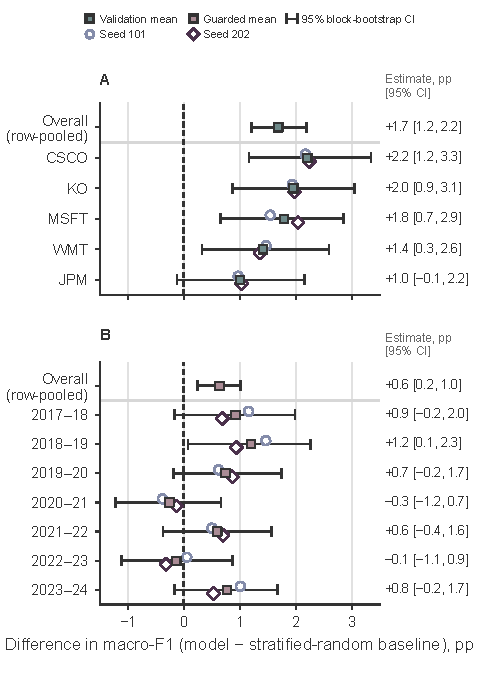
\includegraphics[width=0.66\linewidth]{figures/fig_validation_deltas}
  \Description{A two-panel dot-range plot with a shared horizontal scale from
    -1.5 to +3.5 percentage points. Panel A shows the prespecified validation
    domain with an overall row-pooled estimate followed by ticker rows ordered
    CSCO, KO, MSFT, WMT, and JPM. For each row, a capped whisker spans the
    95 percent block-bootstrap interval, open markers show the two seeds when applicable,
    and a domain-colored filled square shows the two-seed mean; the JPM interval crosses zero.
    Panel B shows the guarded secondary analysis with an overall row-pooled
    estimate followed by periods 2017--18 through 2023--24; five of seven period
    means are positive, two are negative, and six of seven period intervals
    include zero. Dashed zero lines mark no gain over the baseline in both panels,
    and the right column gives each row's estimate and 95 percent block-bootstrap
    interval; these intervals are descriptive, not inferential claims.}
  \caption{Descriptive \macrofone{} deltas for the predeclared TCN primary
  against same-row stratified dummy; positive values favor the model. Panel A
  is prespecified validation by ticker; Panel B is the guarded
  12-month walk-forward. The JPM interval and six of
  seven guarded intervals include zero. Panel B is not a clean test,
  independent holdout, or model-selection ranking.}
  \label{fig:validation_deltas}
\end{figure}
